\providecommand{\main}{../../..}
\documentclass[\main/main.tex]{subfiles}
\begin{document}

\subsection{Esercizio 2}
Si consideri il seguente problema con due indicatori che rappresentano benefici:

\begin{align*}
  \max f_1 = x_1 -x_2 \\
  \max f_2 = x_2      \\
  x_1 + x_2 & \leq 3  \\
  x_1       & \leq 2  \\
  x_1, x_2 \geq 0     \\
\end{align*}

Si determini la soluzione ottima rispetto alla funzione di utilità che combina i
due indicatori con pesi $\w_1 = 1/3$ e $\w_2 = 2/3$.

\subsection{Risoluzione esercizio 2}

\[
  f^* = \frac{1}{3}\rnd{x_1-x_2} + \frac{2}{3}x_2 = \frac{1}{3}\rnd{x_1 + x_2}
\]


\begin{align*}
  \max f_1 = \frac{1}{3}\rnd{x_1 + x_2} \\
  x_1 + x_2 & \leq 3                    \\
  x_1       & \leq 2                    \\
  x_1, x_2 \geq 0                       \\
\end{align*}

Il problema ha soluzione ottima su tutto il segmento tra $A =(2,1)$ e $B = (1,2)$

\subsubsection*{Verifico soluzione}

\begin{figure}
  \begin{subfigure}{0.45\textwidth}
    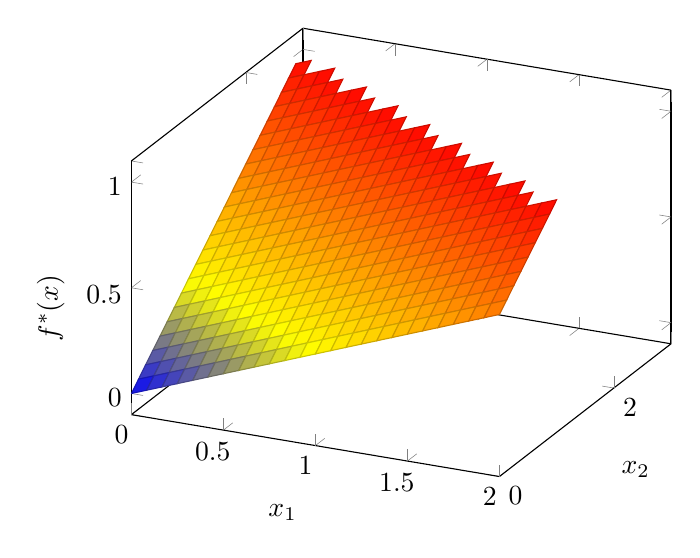
\begin{tikzpicture}
      \begin{axis}[
          xlabel=$x_1$,
          ylabel=$x_2$,
          zlabel=$f^*(x)$,
          domain=0:2,
          y domain=0:3
        ]
        \addplot3[surf, unbounded coords=jump]
        {x+y<=3 ? 1/3*(x+y) : NaN};
      \end{axis}
    \end{tikzpicture}
    \caption{La funzione $f^*(x)$}
  \end{subfigure}
  ~
  \begin{subfigure}{0.45\textwidth}
    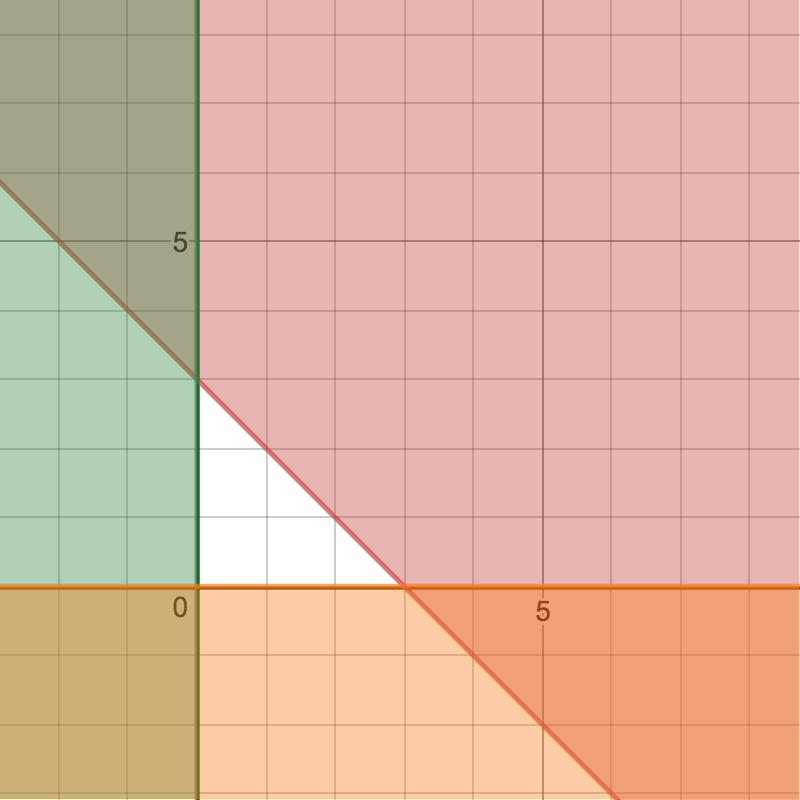
\includegraphics[width=0.8\textwidth]{es2-maut}
    \caption{Dominio della funzione $f^*(x)$}
  \end{subfigure}
\end{figure}

\end{document}